\documentclass[final,20pt]{beamer}
\usepackage{fontenc}
\usepackage{graphicx, float}
\usepackage{geometry}
\usepackage{parskip}

\usepackage{colonequals}
\usepackage{booktabs}
\usepackage{amsmath}
\usepackage{amsthm, amsfonts, amssymb}

% \usepackage[implicit=true]{hyperref}
% \hypersetup{
% hypertexnames = false,
% bookmarksdepth = 2,
% bookmarksopen = true,
% colorlinks,
% linkcolor = blue,
% citecolor = green,
% urlcolor = blue,
% pdfstartview={XYZ null null 1}
% }
\usepackage{bookmark}
% \usepackage[capitalise]{cleveref}

\usepackage{tikz, tikz-cd}
\usetikzlibrary{calc}
\usetikzlibrary{arrows}
\usetikzlibrary{matrix}
\usetikzlibrary{positioning}

% fonts
\usepackage{libertine}
\usepackage[libertine]{newtxmath}
\usepackage{eucal}
\renewcommand*\ttdefault{lmvtt} %monospace font
\usepackage{microtype}
\frenchspacing

%\usepackage[backend=biber, datamodel=mrnumber, maxbibnames=99, sortcites]{biblatex}
%\addbibresource{bibliography.bib}

\usepackage{gitinfo2}

\newcommand\gitfootnote[1]{
  \begin{NoHyper}
  \renewcommand\thefootnote{}\footnote{#1}
  \addtocounter{footnote}{-1}
  \end{NoHyper}
}


% \usepackage{thmtools}
% \declaretheoremstyle[
%   spaceabove = 3pt,
%   spacebelow = 3pt,
%   bodyfont = \itshape,
% ]{first}
% \declaretheoremstyle[
%   spaceabove = 3pt,
%   spacebelow = 3pt,
% ]{second}
% \declaretheorem[numberwithin=section, style=first]{theorem}
% \declaretheorem[sibling=theorem, style=first]{conjecture}
% \declaretheorem[sibling=theorem, style=first]{corollary}
% \declaretheorem[sibling=theorem, style=first]{lemma}
% \declaretheorem[sibling=theorem, style=first]{proposition}

% \declaretheorem[sibling=theorem, style=second]{example}
% \declaretheorem[sibling=theorem, style=second]{remark}
% \declaretheorem[sibling=theorem, style=second]{definition}
% \declaretheorem[sibling=theorem, style=second]{notation}
% \declaretheorem[sibling=theorem, style=second]{assumption}
% \declaretheorem[sibling=theorem, style=second]{convention}
% \declaretheorem[sibling=theorem, style=second]{setup}

% \Crefname{assumption}{Assumption}{Assumptions}
% \Crefname{convention}{Convention}{Conventions}
% \Crefname{setup}{Setup}{Setups}

% \declaretheorem[numberwithin=section, style=first, title=Theorem]{alphatheorem}
% \declaretheorem[sibling=alphatheorem, style=first, title=Conjecture]{alphaconjecture}
% \declaretheorem[sibling=alphatheorem, style=first, title=Question]{alphaquestion}

% \renewcommand{\thealphatheorem}{\Alph{alphatheorem}}
% \renewcommand{\thealphaconjecture}{\Alph{alphaconjecture}}
% \renewcommand{\thealphaquestion}{\Alph{alphaquestion}}
% \crefname{alphatheorem}{Theorem}{Theorems}
% \crefname{alphaconjecture}{Conjecture}{Conjectures}
% \crefname{alphaquestion}{Question}{Questions}



\DeclareMathOperator{\Hom}{Hom}
\DeclareMathOperator{\Ext}{Ext}
\DeclareMathOperator{\GL}{GL}
\DeclareMathOperator{\parameterspace}{R}
\DeclareMathOperator{\modulispace}{M}
\DeclareMathOperator{\Pic}{Pic}
\DeclareMathOperator{\rk}{rk}
\DeclareMathOperator{\Hochschild}{HH}
\DeclareMathOperator{\HH}{H}
\DeclareMathOperator{\hh}{h}


% Numbers
\newcommand{\NN}{\mathbb{N}}
\newcommand{\ZZ}{\mathbb{Z}}
\newcommand{\QQ}{\mathbb{Q}}
\newcommand{\RR}{\mathbb{R}}
\newcommand{\CC}{\mathbb{C}}

% Spaces
\newcommand{\PP}{\mathbb{P}}
% \newcommand{\AA}{\mathbb{A}}


% Sheaves
\DeclareMathOperator{\sheafHom}{\mathscr{H}\kern -2.5pt\mathit{om}}
\DeclareMathOperator{\sheafExt}{\mathscr{E}\mathit{xt}}


% If and only if
\newcommand{\iif}{\ensuremath{\Leftrightarrow}}

% Arrow with optional label.
% Use as A \to[label] B
\renewcommand*{\to}[1][]{\overset{#1}{\rightarrow}}


\newcommand{\stable}{\hyphen\mathrm{st}}
\newcommand{\semistable}{\hyphen\mathrm{sst}}
\newcommand{\tuple}[1]{\ensuremath{\mathbf{#1}}}


\newcommand{\todo}[1]{{\color{blue}#1}}
% ====================
% Packages
% ====================

% \usepackage[T1]{fontenc}
% \usepackage{lmodern}
\usepackage[size=custom, width=76.2, height=101.6, scale=1.0]{beamerposter}
\usetheme{gemini}
\usecolortheme{gemini}
% \usepackage{graphicx}
\usepackage{epstopdf}  % Include the epstopdf package
\usepackage{pgfplots}
\pgfplotsset{compat=1.14}
\usepackage{anyfontsize}
\usepackage{booktabs}


\usepackage[backend=biber, datamodel=mrnumber, maxbibnames=99, sortcites]{biblatex}
\addbibresource{poster.bib}

% ====================
% Lengths
% ====================

% If you have N columns, choose \sepwidth and \colwidth such that
% (N+1)*\sepwidth + N*\colwidth = \paperwidth
\newlength{\sepwidth}
\newlength{\colwidth}
\setlength{\sepwidth}{0.025\paperwidth}
\setlength{\colwidth}{0.3\paperwidth}

\newcommand{\separatorcolumn}{\begin{column}{\sepwidth}\end{column}}

% ====================
% Title
% ====================

\title{Machine learning features of quiver moduli}

\author{Gianni Petrella - University of Luxembourg \inst{1}}

\institute[shortinst]{\inst{1} Work supported by the Luxembourg National Research Fund (AFR-17953441)}
% ====================
% Footer (optional)
% ====================

\footercontent{
  \href{https://giannipetrella.eu}{www.giannipetrella.eu} \hfill
  Princeton ML Theory Summer School - August 12-21, 2025}
  % Computations in Algebra and Geometry, ETH - August 25-29, 2025}

% ====================
% Logo (optional)
% ====================

% Include Eurecom logo on the right side of the header
\logoright{
\includegraphics[height=7cm]{UNI-Logo-en-rgb.png}}
% Include Lab logo on the left side of the header
% \logoleft{\includegraphics[height=7cm]{./logos/s3logo.png}}

% ====================
% Body
% ====================

\begin{document}

\begin{frame}[t]
\begin{columns}[t]
\separatorcolumn

\begin{column}{\colwidth}

  \begin{block}{Representations of quivers}

    A \emph{quiver} $Q$ is a finite directed multigraph with vertices $Q_0$ and arrows $Q_1$.
    A \emph{representation} $V$ of $Q$ is a choice of vector space $V_i$ per vertex $i$
    and a choice of linear application $M_{\alpha}$ for each arrow $\alpha$ \cite{2311.17003}.

    The \emph{dimension vector} of a representation $V$
    is
    \begin{equation*}
    \tuple{d} \colonequals \dim(V) \colonequals (\dim(V_i))_{i \in Q_0}.
    \end{equation*}

    \begin{figure}
      \centering
      \begin{tikzpicture}
        \node (1) at (0, 0)              {$\bullet$};
        \node (4) [above of = 1]              {$1$};
        \node (2) at (6, 0)              {$\bullet$};
        \node (5) [above of = 2]               {$3$};
        \node (3) at (6, -6)             {$\bullet$};
        \node (6) [above of = 3]              {$5$};

        \draw[->, bend left  = 30] (1) edge (2);
        \draw[->, bend left  = 10] (1) edge (2);
        \draw[->, bend right = 10] (1) edge (2);
        \draw[->, bend right = 30] (1) edge (2);
        \draw[->, bend left  = 10] (1) edge (3);
        \draw[->, bend right = 10] (1) edge (3);
        \draw[->]                  (2) edge (3);
      \end{tikzpicture}
      \caption{A quiver with three vertices.}
    \end{figure}

    A representation is, equivalently, a point
    in the \emph{representation space}
    \begin{equation}
      \repspace(Q, \tuple{d}) \colonequals \bigoplus_{\alpha \in Q_1} \operatorname{Mat}_{d_{t\alpha, s\alpha}}(\CC)
    \end{equation}

    Two representations are \emph{isomorphic} if they are equivalent up to
    a change of basis -
    that is, if they lie in the same orbit of the action
    of $\GLd$ on $\repspace(Q, d)$.

    If one fixes a \emph{stability parameter} $\theta \in \ZZ^{Q_0}$ that satisfies
    the identity~$\theta\cdot\tuple{d}=0$, we say that a representation $V$
    is $\theta$-stable, respectively $\theta$-semistable,
    if every subrepresentation $W \subset V$ satisfies
    $\theta \cdot \dim(W) < 0$, respectively
    $\theta\cdot\dim(W)\leq 0$.

  \end{block}

  \begin{block}{Moduli spaces of stable representations}

    The sets of $\theta$-stable and semistable representations
    are GIT-stable opens in $\repspace(Q, \tuple{d})$.
    We can thus consider their GIT quotients.

    The relations between the affine, semistable and stable quotients are summarised in the following diagram:
    \begin{equation}
      \begin{tikzcd}[row sep=small, column sep=small, ampersand replacement=\&]
        \repspace^{\theta\stable}(Q, \tuple{d}) \arrow[r,hook] \arrow[d]     \& \repspace^{\theta\semistable}(Q, \tuple{d}) \arrow[r,hook] \arrow[d]     \& \repspace(Q, \tuple{d}) \arrow[d] \\
        \repspace^{\theta\stable}(Q, \tuple{d})\gitquot\GLd \arrow[r, hook] \arrow[d, equal] \& \repspace^{\theta\semistable}(Q, \tuple{d})\gitquot\GLd \arrow[r, two heads] \arrow[d, equal] \& \repspace(Q, \tuple{d}) / \GLd \arrow[d, equal] \\
        \modulispace^{\theta\stable}(Q, \tuple{d}) \arrow[r, hook]          \& \modulispace^{\theta\semistable}(Q, \tuple{d}) \arrow[r, two heads]                \& \modulispace^{\semisimple}(Q, \tuple{d}).
      \end{tikzcd}
    \end{equation}

    It is known that horizontal inclusions are open and surjections are projective.
    Moreover, the moduli of stable representations is smooth, and
    $\mathcal{O}(\modulispace^{\semisimple}(Q, d))$ is generated by traces of products over
    oriented cycles in $Q$ \cite{MR958897}.
    If $Q$ is acyclic, $\modulispace^{\semisimple}(Q, d)$ is thus a point
    and $\modulispace^{\theta\semistable}(Q, d)$ is a projective variety.

    The complement of $\repspace^{\theta\semistable}(Q,\tuple{d})$ is the
    \emph{unstable locus}. It admits a stratification into locally closed
    subsets, called \emph{Harder--Narasimhan strata}.
  \end{block}

  \begin{alertblock}{Geometric invariants}

    Many geometric invariants of quiver moduli can be computed effectively
    using the software package \quivertools~\cite{quivertools,2506.19432}.
    However, complexity is often a limiting factor,
    so for large scale applications we attempt to model
    several of these features using machine learning techniques.

    \begin{itemize}
      \item \textbf{Euler characteristic} is obtained
      via Betti numbers computations \cite{MR1974891}.
      These are strong topological invariants of complex varieties,
      and appear in many different mathematical settings.

      \item \textbf{Teleman inequality ratios} are numbers between $0$ and $1$ defined
      on each Harder--Narasimhan stratum of $\repspace(Q,\tuple{d})$.
      If all of them are strictly smaller than $1$,
      \emph{Teleman quantization} can be applied to show higher cohomology vanishings
      on $\modulispace^{\theta\semistable}(Q,\tuple{d})$.
      This is done in detail in \cite{2311.17003}.
    \end{itemize}

  \end{alertblock}
\end{column}

\separatorcolumn

\begin{column}{\colwidth}


  \begin{block}{Datasets}
    The training data is obtained by classical algorithms derived from
    the literature of quiver representations. These are implemented in
    \quivertools, see \cite{quivertools} and the accompanying \cite{2506.19432}.
    We harvested data by running the Julia version of \quivertools~on a cluster,
    using {\tt{Distributed.jl}} to parallelize the computations across 128 cores,
    for a total CPU time of ~1000h.
    For this work, we use a set of 50000 combinations of 4-vertex quivers
    and dimension vectors $\tuple{0} \leq \tuple{d}\leq(5, 5, 5, 5)$.
    For the Euler characteristic prediction, we ran experiments
    exclusively with dimension vector $(1, 1, 1, 1)$.
    These are mathematically relevant because the resulting quiver moduli
    are toric varieties.
  \end{block}

  \begin{block}{Methodology}

    We train feedforward neural networks to predict various numerical values
    associated to a quiver and a dimension vector.
    For all of our prediction problems we use multi-layer perceptron architectures.
    The input of our network is always the adjacency matrix of the quiver, flattened,
    joined to the dimension vector.
    The dataset is split into training (80\%) and testing data (20\%).

    We use {\tt{Flux.jl}} \cite{flux.jl,innes:2018}, a pure Julia ML stack.

   \begin{figure}
      \centering
      \begin{tikzpicture}[
      neuron/.style={circle, fill=black!25, minimum size=30pt, inner sep=0pt},
          input neuron/.style={neuron, fill=green!50},
          output neuron/.style={neuron, fill=red!50},
          hidden neuron/.style={neuron, fill=blue!50},
      ]
        \node[input neuron] (1-0) at (0,0) {};
        \node[input neuron] (1-1) at (0,2) {};
        \node             (1-mid) at (0,4) {\vdots};
        \node[input neuron] (1-2) at (0,6) {};
        \node[input neuron] (1-3) at (0,8) {};

        \node[hidden neuron] (2-0) at (3,-1) {};
        \node[hidden neuron] (2-1) at (3, 1) {};
        \node[hidden neuron] (2-2) at (3, 3) {};
        \node              (2-mid) at (3, 4) {\vdots};
        \node[hidden neuron] (2-3) at (3, 5) {};
        \node[hidden neuron] (2-4) at (3, 7) {};
        \node[hidden neuron] (2-5) at (3, 9) {};

        \foreach \source in {0,...,3}
          \foreach \target in {0,...,5}
            \draw[->] (1-\source) edge (2-\target);

        \node (3-0) at (6,-1) {\dots};
        \node (3-1) at (6, 1) {\dots};
        \node (3-2) at (6, 3) {\dots};
        \node (3-3) at (6, 5) {\dots};
        \node (3-4) at (6, 7) {\dots};
        \node (3-5) at (6, 9) {\dots};

        \foreach \source in {0,...,5}
          \foreach \target in {0,...,5}
            \draw[->] (2-\source) edge (3-\target);

        \node[hidden neuron] (4-0) at (9,-1) {};
        \node[hidden neuron] (4-1) at (9, 1) {};
        \node[hidden neuron] (4-2) at (9, 3) {};
        \node              (4-mid) at (9, 4) {\vdots};
        \node[hidden neuron] (4-3) at (9, 5) {};
        \node[hidden neuron] (4-4) at (9, 7) {};
        \node[hidden neuron] (4-5) at (9, 9) {};

        \foreach \source in {0,...,5}
          \foreach \target in {0,...,5}
            \draw[->] (3-\source) edge (4-\target);


        \node[hidden neuron] (5-0) at (12,-1) {};
        \node[hidden neuron] (5-1) at (12, 1) {};
        \node[hidden neuron] (5-2) at (12, 3) {};
        \node              (5-mid) at (12, 4) {\vdots};
        \node[hidden neuron] (5-3) at (12, 5) {};
        \node[hidden neuron] (5-4) at (12, 7) {};
        \node[hidden neuron] (5-5) at (12, 9) {};

        \foreach \source in {0,...,5}
          \foreach \target in {0,...,5}
            \draw[->] (4-\source) edge (5-\target);

        \node[output neuron] (6) at (15, 4) {};

        \foreach \source in {0,...,5}
          \draw[->] (5-\source) edge (6);

        \end{tikzpicture}
      \caption{A standard feedforward neural network. Input neurons are in green, and
      the output neuron is in red.}
    \end{figure}

    Current results are based on the following choices of hyperparameters.
    We implemented a decay scheme that halves the learning rate
    whenever it detects a plateau in the training loss lasting for at least 30 epochs.
    Our models were let train for 1000 epochs.

    \begin{table}
      \centering
      \begin{tabular}{lcc}
        \toprule
        Hyperparameter & Euler characteristic & Teleman ratio\\
        \midrule
        Hidden layers             & 3                   & 3\\
        Layer sizes               & (4096, 4096, 1024)  & (4096, 4096, 512)\\
        Activations               & {\tt{relu}}         & {\tt{relu}}, sigmoid\\
        Learning rate             & $10^{-4}$           & $5 \cdot 10^{-5}$\\
        Optimiser                 & Adam                & Adam\\
        Loss function             & least squares       & least squares\\
        \bottomrule
      \end{tabular}
      \caption{Hyperparameters used in current setup.}
    \end{table}


  \end{block}

  \begin{block}{Results}

    In all of our problems we were able to achieve high precision in predicting
    numerical invariants.
    Our model predicting Teleman ratios achieves an average loss of
    $<0.005$ on training data and $<0.03$ on test data.

    \phantom{a}

    \begin{figure}
    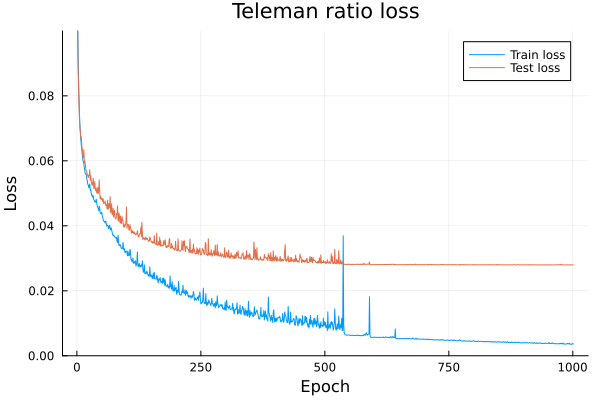
\includegraphics{teleman-ratio-loss.png}
    \caption{Loss of Teleman ratio predictor over training.}
    \end{figure}
  \end{block}

\end{column}

\separatorcolumn

\begin{column}{\colwidth}
  \begin{block}

    Our model predicting Euler characteristics scores
    $>85\%$ on training data and $~80\%$ on test data,
    with both train and test losses being $<0.5$.

    \begin{figure}
    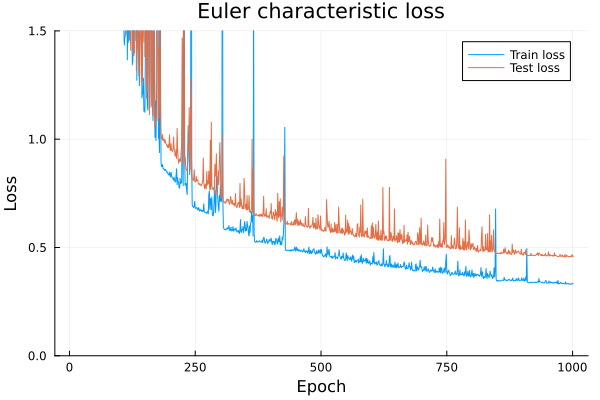
\includegraphics{chi-loss.png}
    \caption{Loss of Euler characteristic prediction over training.}
    \end{figure}

    \begin{figure}
    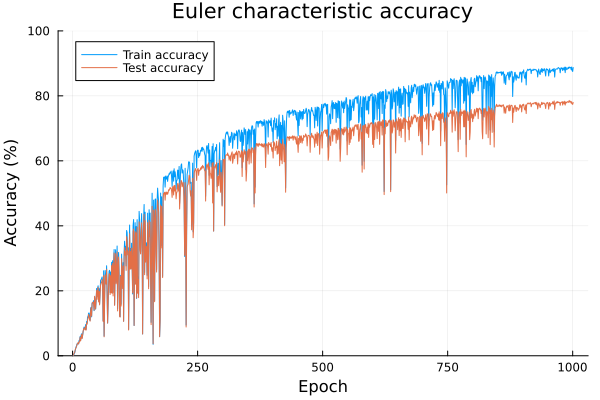
\includegraphics{chi-accuracy.png}
    \caption{Accuracy of Euler characteristic prediction over training.}
    \end{figure}

    \end{block}

  \begin{exampleblock}{Conclusions}

    Our work shows that relatively simple mathematical methods
    can reliably approximate invariants previously known to only be accessible
    via highly complex algorithms.

    On one hand, this suggests that less complex algorithms
    may exist, and further research in this direction might be fruitful.

    On the other hand, our results serve as evidence
    to the usefulness of ML-enabled workflows for mathematical research:
    as we have proved that our features are learnable,
    we plan to use more sophisticated workflows for generating
    mathematically meaningful examples, e.g. using
    transformer networks via PatternBoost \cite{2411.00566}.
  \end{exampleblock}

  % \begin{block}{Outlook}

  %   PatternBoost is a ML-enabled mathematical research workflow
  %   presented in .
  %   It consists of two iterative phases:
  %   a classical search for mathematical objects
  %   and their properties conducted using classical algorithms,
  %   and a training phase
  %   in which the best results of the search
  %   are used to train a transformer neural network.
  %   Samples from the trained transformer are
  %   then used as starting point for the search phase again,
  %   and the process repeats.

  %   PatternBoost has been used to produce examples of mathematical objects
  %   that maximize certain quantities, namely exceeding conjectured bounds
  %   and thus disproving standing conjectures (see \cite[Section~3.3]{2411.00566}).

  %   \todo{add a scheme explaining PatternBoost}

  %   We plan to apply the PatternBoost technique to search for quiver moduli
  %   that optimise currently open problems, e.g. in \cite{2311.17003}.
  % \end{block}

  \begin{block}{References}

  {\footnotesize
  \printbibliography
}
  \end{block}

\end{column}

\separatorcolumn
\end{columns}
\end{frame}

\end{document}
